\documentclass[a4paper,12pt]{article}


\usepackage[utf8x]{inputenc}
\usepackage[T2A]{fontenc}
\usepackage[english, russian]{babel}
\usepackage{pdfpages}

% Опционно, требует  apt-get install scalable-cyrfonts.*
% и удаления одной строчки в cyrtimes.sty
% Сточку не удалять!
% \usepackage{cyrtimes}

% Картнки и tikz
\usepackage{graphicx}
\usepackage{tikz}
\usetikzlibrary{snakes,arrows,shapes}


% Некоторая русификация.
\usepackage{misccorr}
\usepackage{indentfirst}
\renewcommand{\labelitemi}{\normalfont\bfseries{--}}

% Увы, поля придётся уменьшить из-за листингов.
\topmargin -1cm
\oddsidemargin -0.5cm
\evensidemargin -0.5cm
\textwidth 17cm
\textheight 24cm

\sloppy

% Оглавление в PDF
\usepackage[
bookmarks=true,
colorlinks=true, linkcolor=black, anchorcolor=black, citecolor=black, menucolor=black,filecolor=black, urlcolor=black,
unicode=true
]{hyperref}

% Для исходного кода в тексте
\newcommand{\Code}[1]{\texttt{#1}}

\usepackage{verbatim}
\usepackage{fancyvrb}
\fvset{frame=leftline, fontsize=\small, framerule=0.4mm, rulecolor=\color{darkgray}, commandchars=\\\{\}}
\renewcommand{\theFancyVerbLine}{\small\arabic{FancyVerbLine}}


\title{ Курсовая работа по дисциплине \\ "Протоколы вычислительных сетей" \\ <<SMTP клиент, 31 вариант>>}
\author{Сёмина Валерия Алексеевна ИУ7-37}

\begin{document}


\maketitle

\tableofcontents

\section{Введение}

В ходе выполнения данного курсового проекты был разработан SMTP клиент.
Выполнены все требования, предъявляемые к реализации, а именно:

\begin{Verbatim}
1. Используется вызов select и единственный рабочий процесс (поток).
2. Журналирование производится в отдельном процессе.
3. Пытаться отправлять все сообщения для одного MX за одну сессию.
\end{Verbatim}

\section{Аналитический раздел}

\subsection{Анализ требований к реализации}

Для отслеживания поступления новых файлов (сообщений) используется системный вызов \textbf{select}. Данный вызов блокирует выполяющийся поток до того момента, как не появятся данные на каком-либо из соединений. Это позволяет отслеживать одновременно несколько дескрипторов. Таким образом, при поступлении новых писем в директорию, срадабывает системный вызов и процесс выходит из состония блокировки и продолжает выполнение.

Однако системный вызов \textbf{select} имеет некоторое ограничение, он позволяет отслеживать изменение состояния только первых 1024 файловых дескрипторов.

\subsection{Сущности предметной области}
Анализ предметной области позволил выявить следующие необходимые сущности:
\begin{itemize}
\item письмо;
\item получатель;
\item отправитель;
\item домен;
\item тело письма;
\item заголовок письма
\end{itemize}

Зависимость между сущностями предметной области отображена на диаграмме ~\ref{fig:er_mail}

\begin{figure}[h]
\centering
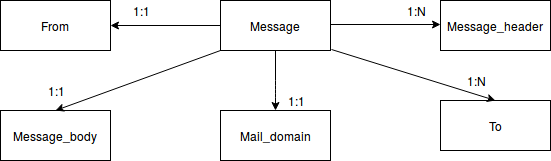
\includegraphics[width=0.6\textwidth]{includes/er_mail.png}
\caption{ER-диаграмма}
\label{fig:er_mail}
\end{figure}

\subsection{Метод хранения писем в программе}
Все письма хранятся в одном списке. Когда в директории появляются новые файлы, из них формируется список и отправляется на обработку.

\section{Конструкторский раздел}

\subsection{Конечный автомат состояния SMTP - клиента}
На рисунке ~\ref{fig:fsm} представлен конечный автомат, описывающие возможные состояния SMTP - клиента и переходы между этими состояниями.

\begin{figure}[h]
\centering
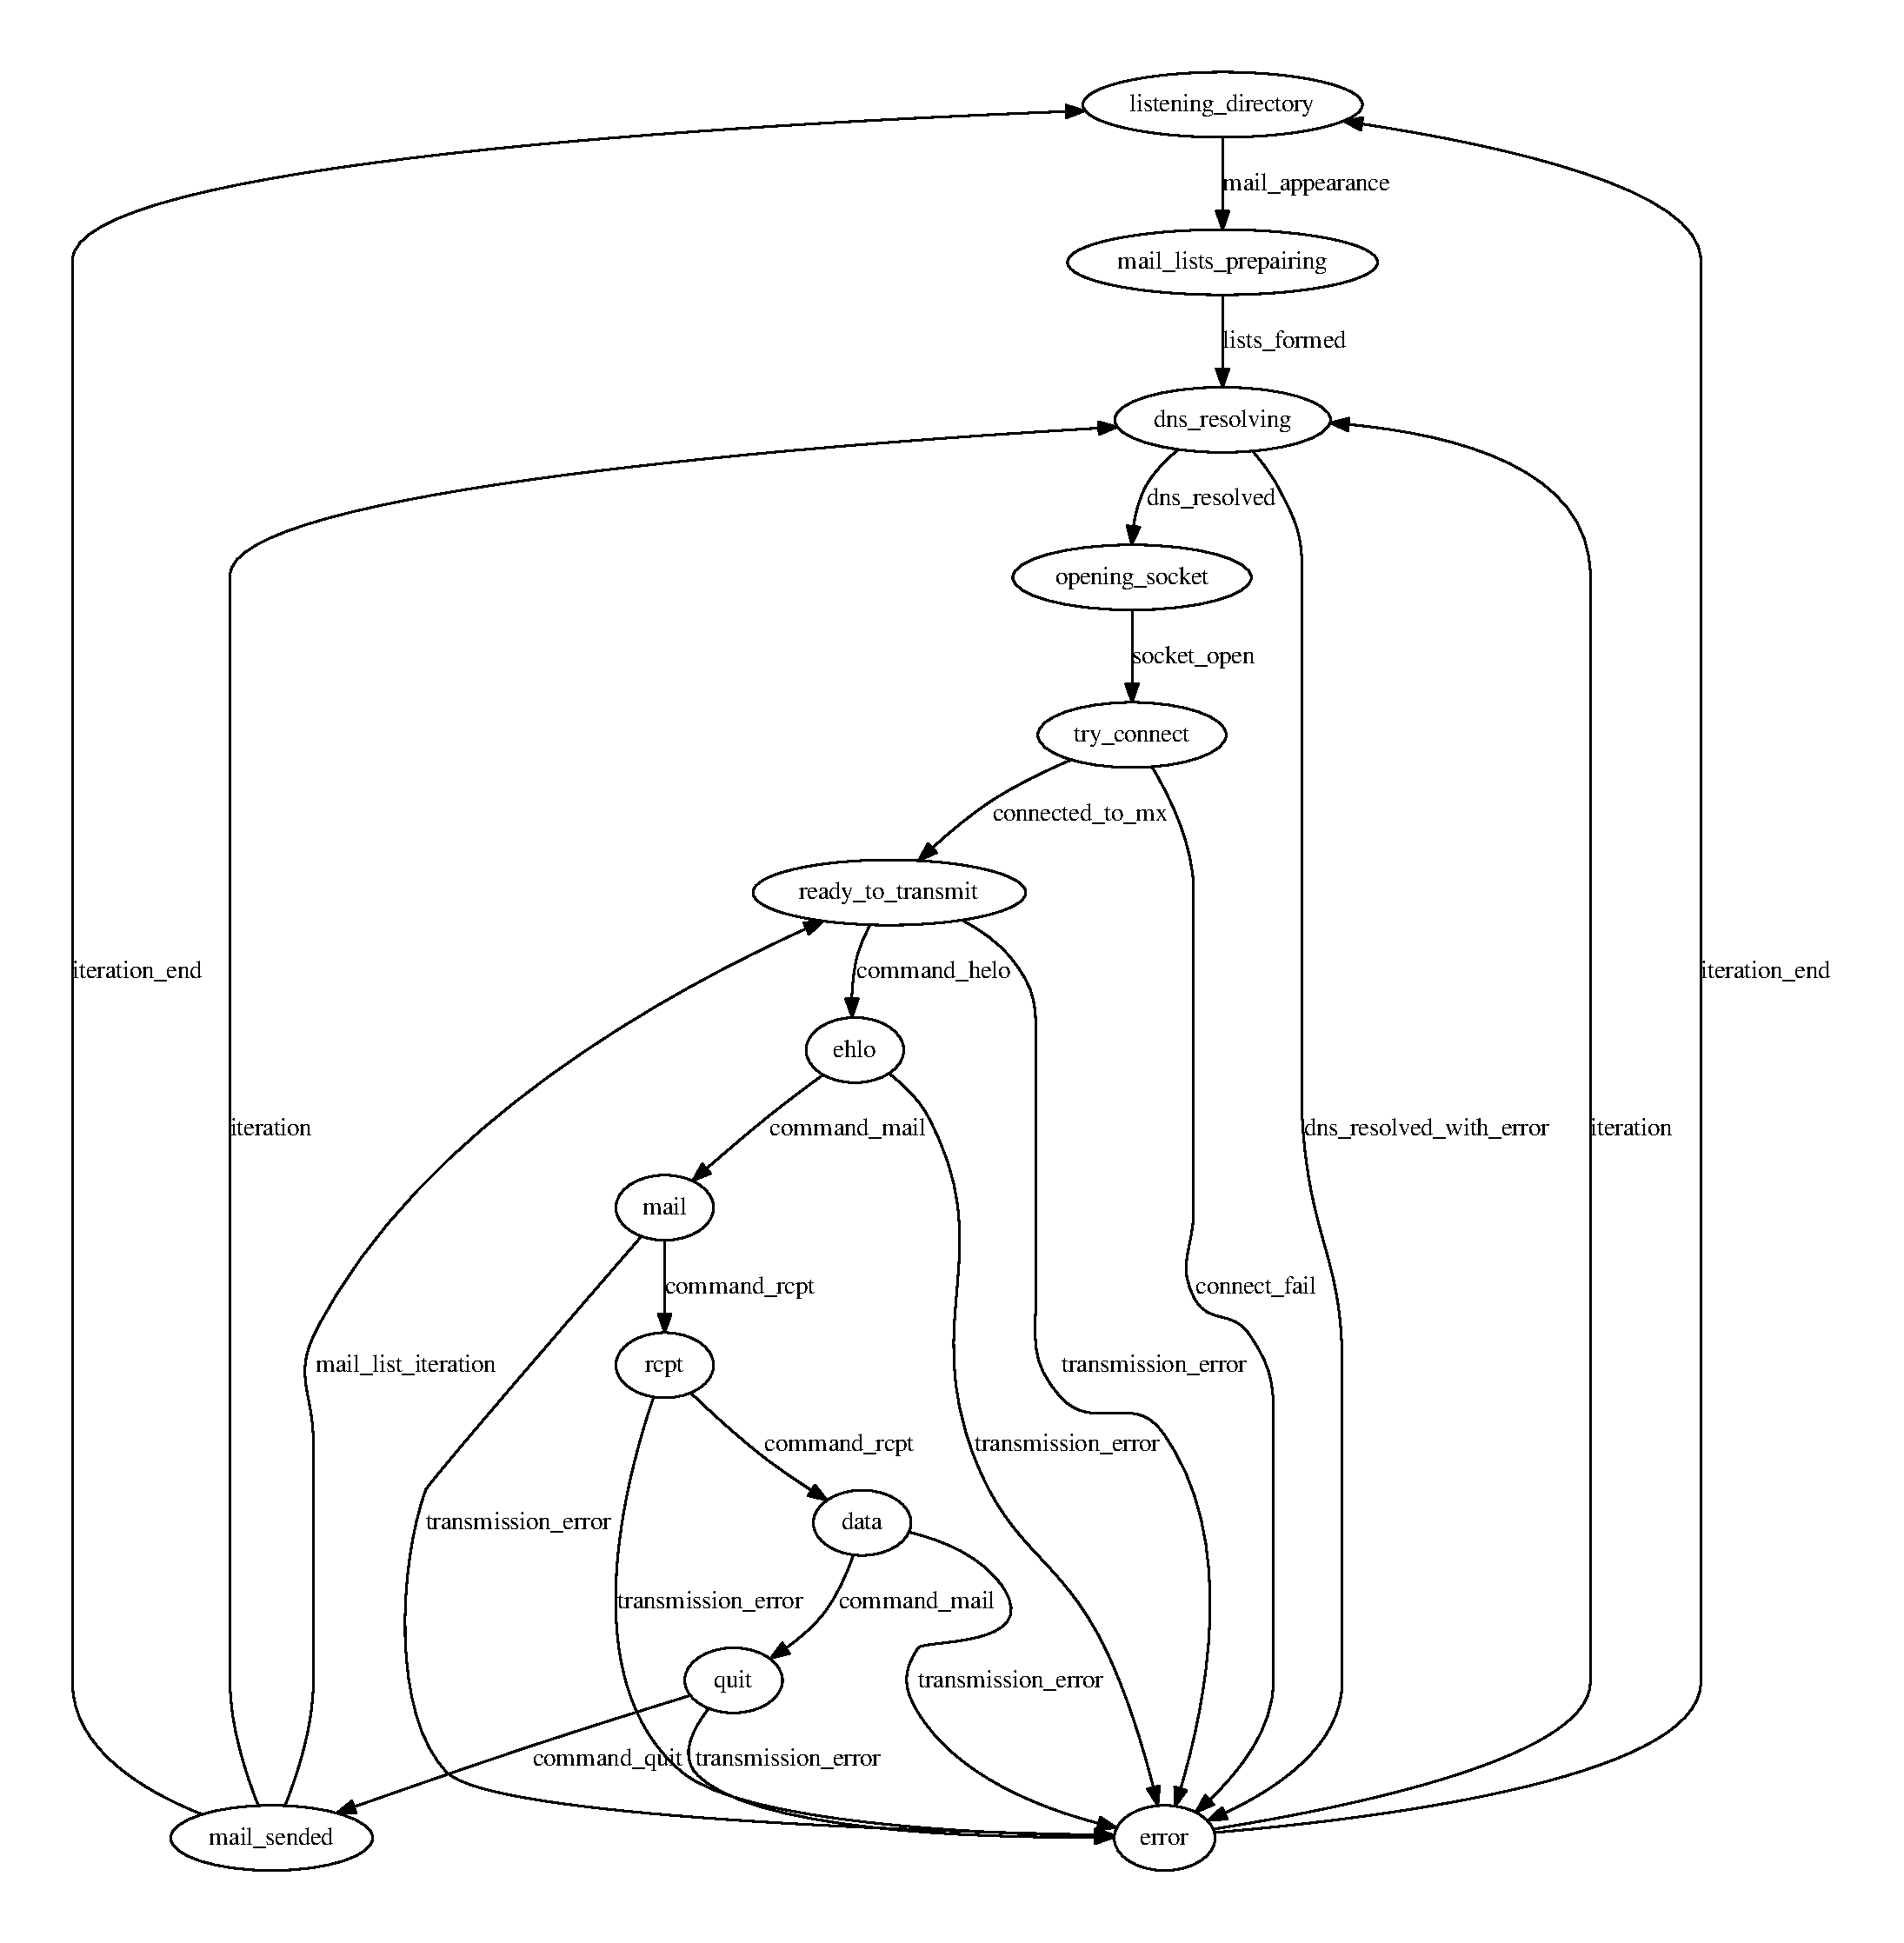
\includegraphics[width=1.0\textwidth]{includes/client_fsm.pdf}
\caption{ER-диаграмма}
\label{fig:fsm}
\end{figure}

\subsection{Синтаксис команд протокола}
SMTP клиент отправляет команды следующие команды:
\begin{itemize}
\item EHLO <имя клиента> - команда приветствия, с которой начинается установка соединения;
\item MAIL FROM: <from address> - от кого пришло письмо;
\item RCPT TO: <to addredd> - кому предназначается письмо, команда отправляется для каждого адреса в отдельности;
\item DATA - начало отправки самого письма;
\item Отправка письма (тело + заголовки);
\item QUIT - команда, закрывающая соединение.
\end{itemize}

SMTP - клиент получается ответ от сервера в виде строки, которая содержт код завершения запроса. В данном случае в решулярных выражениях нет
необходимости. Для получения этого статуса используется функция \textbf{strtol} из стандартной библиотеки языка С. 

\subsection{Ипользуемые структуры данных}

Диаграмма связей между основными структурами данных представлена на рисунке ~\ref{fig:data_structures}

\begin{figure}[h]
\centering
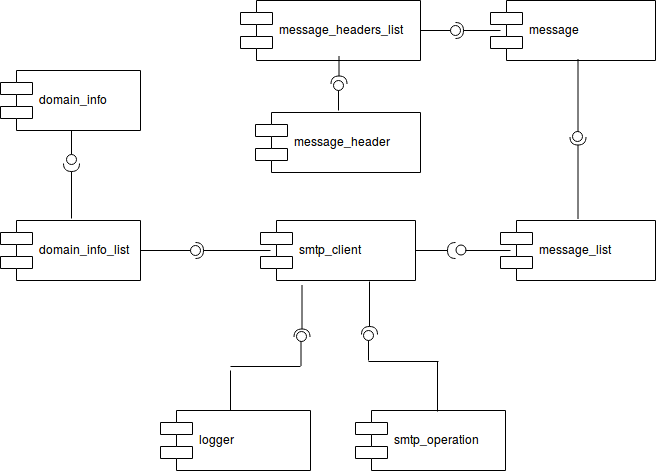
\includegraphics[width=0.8\textwidth]{includes/component_smtp_client.png}
\caption{Диаграмма связей между основными структурами данных}
\label{fig:data_structures}
\end{figure}

\subsection{Выделенные подсистемы}

В ходе анализа возможной архитектуры проектируемого решения было выделено 3 подситемы:

\begin{itemize}
\item файловая подсистема, которая является внешней по отношению к разрабатываемому приложению;
\item подсистема мониторинга файловой системы;
\item подсистема отправки писем.
\end{itemize}

\subsection{Алгоритм работы SMTP - клиента}

На рисунке ~\ref{fig:alg_smtp} представлен алгоритм работы STMP - клиента.

\begin{figure}[h]
\centering
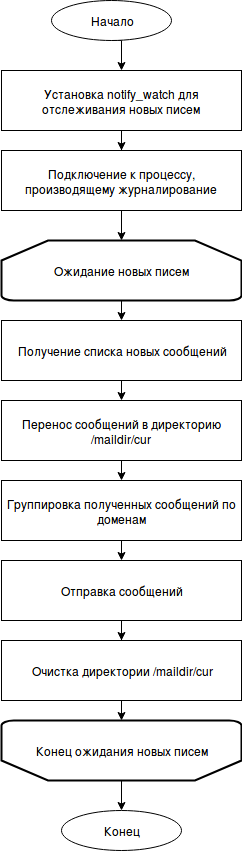
\includegraphics[width=0.3\textwidth]{includes/alg_smpt.png}
\caption{Алгоритм работы SMTP - клиента}
\label{fig:alg_smtp}
\end{figure}

Из диаграммы, представленной выше, видно, что сначала осуществляется установка мониторинга за директорией \textbf{/maildir/new}, куда
поступают новые сообщения. Затем, процесс блокируется на системной вызове \textbf{select} до того момента, когда в указанной выше директории
появляются новые письма. Только что поступившие сообщения перемещаются в \textbf{/maildir/cur} и отправляются в обработку, а именно,
группируются по доменам и отслылаются. Отправка для одного домена осуществляется в рамках одной сессии. После отправки писел директория \textbf{/maildir/cur} очищается.

\subsection{Алгоритм поключения к сокету}

На рисунке ~\ref{fig:connect_alg} представлен алгоритм подключения по сокету к SMTP - серверу домена.

\begin{figure}[h]
\centering
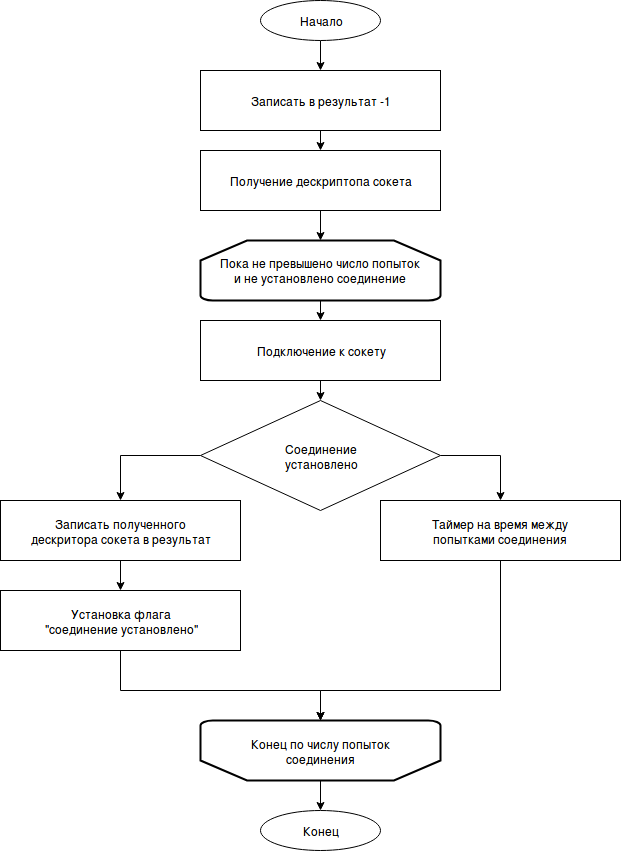
\includegraphics[width=0.8\textwidth]{includes/connect_alg.png}
\caption{Алгоритм работы SMTP - клиента}
\label{fig:connect_alg}
\end{figure}

Поключение осуществляется по установенному максимальному числу попыток со временем между попытками в случае неуспешного предыдущего подключения.


\subsection{Inter Process Communications (IPC)}
Так как журналирование, согласно требованиям курсовго проекта, должно проводиться в отдельно процессе, следовательно,
необходимо организовать взаимодействие основного процесса SMTP - клиента и процесс, осуществляющего логгирование.
Для этой цели был выбран механизм \textbf{POSIX MQ}.
Оба процессы общаются с использованием одной известной очереди сообщений. SMTP - клиент отправляет сообщение в очередь, процесс, ведущий журанилирование,
извлекает последнее поступившее в очередь сообщение и записывает его в журнал.

\subsection{Механизм хранения почты}
Для хранения почты и разделения доступа к файлам используется структура \textbf{Maildir}. Структура следующая: поддиректория \textbf{new} - содержит новые, только что поступившие письма, поддиректория \textbf{cur} - содержит письма, взятые в обработку.
Как только в \textbf{new} появляется файл/файлы, подсистема мониторинга входящей почты перемещает его/их в поддиректорию \textbf{cur}, откуда уже, в свою очередь, файлы берутся на обработку.

\subsection{Входные данные для SMTP - клиента}
\begin{itemize}
\item Пусть к поддиректории new директории maildir;
\item Пусть к поддиректории cur директории maildir;
\item Название очереди сообщения для IPC;
\item Права доступа для создания вышеуказанной очереди;
\item Число попыток подключения к сокету;
\item Время между двумя попытками подключения.
\end{itemize}

\subsection{Входные данные для процесса, осуществляющего журналирование}
\begin{itemize}
\item Название очереди сообщения для IPC;
\item Полное имя файла логирования.
\end{itemize}

\section{Технологический раздел}
\subsection{Генерация кода и сборка}

Сборка проекта осуществляется с помощью утилиты \textbf{GNU Make}. Для данной утилиты были подготовлены makefile. Для кода, отчета и тестов существует свой собственный makefile, также имеется основной makefile, который управляет сборкой всего проекта включая отчет и тесты.
Отчеты, сгенерированные по тестам помещаются в отдельную папку, откуда они уже вставляются в отчет.

Соответственно, существует несколько целей сборки:
\begin{itemize}
\item сборки ПО;
\item сборки отчета;
\item сборки тестов и отчетов по данным тестам.
\end{itemize}

\subsection{CFlow проекта}
Ниже приведен граф зависимостей проекта по функциям, полученный путем генерации с помощью утилиты \textbf{cflow}.
\VerbatimInput{includes/cflow.txt}

\subsection{Модульное тестирование}
В качестве библиотеки для организации модульного тестирования используется библиотека \textbf{CUnit}. Тесты группируются в suites, для выполнения проверок внутри тестов используются предоставляемые библиотекой макросы.

\subsection{Системное тестирование}

Для реализации системного тестирования использовался \textbf{bash} скрипт.
Пример скрипта для организации тестирования представлен ниже:
\begin{Verbatim}
#!/bin/bash

make SystemTests
gnome-terminal -x ./start_logger.sh --disable-factory & pid_logger=$!
gnome-terminal -x ./start_client.sh --disable-factory & pid=$!

sleep 2
cp ./maildir/message.txt ./maildir/new/message.txt
\end{Verbatim}

\subsection{Итоги тестирования}

\textbf{Unit тесты}
\VerbatimInput{includes/UnitTests.txt}

\textbf{Valgrind unit тестов}
\VerbatimInput{includes/valgrind_UnitTests.txt}

\textbf{Системные тесты}
\VerbatimInput{includes/SystemTests.txt}

\textbf{Valgrind системных тестов}
\VerbatimInput{includes/valgrind_SystemTests.txt}

\subsection{Doxygen проекта}

Результат автоматической генерации документации по исходному кода проекта представлен на рисунках ~\ref{fig:struct_domain_info},
~\ref{fig:struct_domain_info_list}, ~\ref{fig:struct_message}, ~\ref{fig:struct_message_headers_list}, ~\ref{fig:struct_message_list} 
и ~\ref{fig:struct_string_list}.

\begin{figure}[h]
\centering
\includegraphics[width=0.8\textwidth]{doxygen/latex/structdomain__info__coll__graph.pdf}
\caption{Структура domain info}
\label{fig:struct_domain_info}
\end{figure}

\begin{figure}[h]
\centering
\includegraphics[width=0.8\textwidth]{doxygen/latex/structdomain__info__list__coll__graph.pdf}
\caption{Структура domain info list}
\label{fig:struct_domain_info_list}
\end{figure}

\begin{figure}[h]
\centering
\includegraphics[width=0.8\textwidth]{doxygen/latex/structmessage__coll__graph.pdf}
\caption{Структура message}
\label{fig:struct_message}
\end{figure}

\begin{figure}[h]
\centering
\includegraphics[width=0.8\textwidth]{doxygen/latex/structmessage__headers__list__coll__graph.pdf}
\caption{Структура message headers list}
\label{fig:struct_message_headers_list}
\end{figure}

\begin{figure}[h]
\centering
\includegraphics[width=0.8\textwidth]{doxygen/latex/structmessage__list__coll__graph.pdf}
\caption{Структура message list}
\label{fig:struct_message_list}
\end{figure}

\begin{figure}[h]
\centering
\includegraphics[width=0.8\textwidth]{doxygen/latex/structstring__list__coll__graph.pdf}
\caption{Структура string list}
\label{fig:struct_string_list}
\end{figure}

\section{Заключение}
В ходе выполнения данного курсового проекты был разработан SMTP клиент.
Выполнены все требования, предъявляемые к реализации, а именно:

\begin{Verbatim}
1. Используется вызов select и единственный рабочий процесс (поток).
2. Журналирование производится в отдельном процессе.
3. Пытаться отправлять все сообщения для одного MX за одну сессию.
\end{Verbatim}

Также были разработаны модульные тесты с использованием библиотеки \textbf{CUnit} и системные тесты с помощью \textbf{bash} скриптов.

\end{document}
